\ProvidesFile{ch-introduction.tex}[2021-01-04 introduction chapter]

\chapter{INTRODUCTION}

Draizelle Sexon \cite{sexon2012} recommends using these chapter names:\\
\I2 Problem and Its Background\\
\I2 Review of Related Literature and Studies\\
\I2 Methodology of the Study\\
\I2 Presentation, Analysis and Interpretation of Data\\
\I2 Summary, Conclusions, and Recommendations

Mantian Xue's \cite{xue2019} thesis contained these chapters:\\
\I2 Introduction\\
\I2 Device Technology\\
\I2 Graphene-based Biosensors\\
\I2 Graphene-based Ion Sensing\\
\I2 MoS${}_2$-based Sensors\\
\I2 Conclusion and Future Work

I suggest thinking carefully about the structure of your thesis
and using appropriate chapter names.


\section{English-related information}


\subsection{Typographic Conventions}

{
  \newlength{\Parindent}
  \setlength{\Parindent}{\parindent}
  \newcommand{\Indent}{\advance\leftskip by \Parindent}
  \parindent = 0pt

  \newcommand{\Describe}[2]{%
    {\Indent \Indent #1\endgraf}%
    {\Indent \Indent \Indent #2\endgraf}%
  }

  {\Indent The following typographic conventions are used in this document.
    These conventions were influenced by \cite{wireshark-users-guide,dijk2000,weh2016}.\endgraf}

  % Admonitions information is in \cite{wireshark-users-guide}.
  % Admonitions are not supported yet.

  % Dialog and window buttons information is in \cite{wireshark-users-guide}.
  % Dialog and window buttons are not supported yet.

  \Describe
  {\Emph{Emphasis}, \First{First Use}, and \Title{Title}}
  {%
    Emphasis: You \Emph{must} do this.\\
    First Use: The first use of an unusual term is \First{emphasized}.
    It is defined soon after it is emphasized.
    The sensor was installed in an \First{ekayak}.
    An ekayak is an electric kayak,
    we used a Duke Energy model
    % A digit dash is used to separate digits---it's the same width as a digit.
    % From http://everets.org/kevin/ten-codes.php retrieved on 2020-02-28:
    %     CODE  MEANS
    %     10-7  Out of service
    % So, the model number is a joke.
    10\FigureDash 7
    for this research.\\
    Title: He read \Title{The Grapes of Wrath}
    and watched \Title{Citizen Kane}.%
  }

  \Describe
  {\Keys{Keyboard} \Keys{Keys}}
  {%
    \Keys{Control + A} means press the Control key and A key at the same time.
    \Keys{A} \Keys{B} means press key A and then press key B.%
  }

  \Describe
  % Can't use \verb iside an arguement to \Describe.
  {{\tt Literal Elements}}
  {%
    Literal elements include checkboxes,
    code,
    environment variables,
    file names,
    function names,
    \LaTeX\ input,
    output,
    variable names,
    and verbatim input (except for commands typed on the command line).
  }

  \Describe
  {\Menu{Menu > Items}}
  {%
    To make sure smooth scrolling is on go to
    \Menu{Open menu > Preferences}
    and make sure the
    {\tt Use smooth scrolling}
    checkbox is checked.%
  }

  \Describe
  {\Place{Placeholders}}
  {Placeholders need to be replaced with real input.}
  
  \Describe
  {\Shell{\ttfamily\bfseries shell commands}}
  {Commands typed on the command line by the user.}
  
}


\subsection{Logical punctation}

I use logical punctuation \cite{yagoda2011}:\\
  \I2 The sign said ``Buses Only''.\\
instead of\\
  \I2 The sign said ``Buses Only.''\\
so quoted material,
and only quoted material,
is inside quotes.
This is new and not many people use it.
Your major professor may not like this style.
Check with them before you decide to use this.


\subsection{Serial comma}

I use the serial comma:\\
  \I2 apple, berry, and cherry\\
instead of\\
  \I2 apple, berry and cherry\\
because I find it easier
to see the list items
when they are separated by commas.





I like
to start all chapter names with \verb+ch-+.
Chapter names are everything
from the beginning of the thesis through the last chapter.
Chapters include all front matter
in addition to all chapters.

Appendices start with \verb+ap-+ and are everything after the last chapter
including any bibliography,
colophon,
indices,
and vita.

Graphics files start with \verb+gr-+.

\paragraph{A new Paragraph}

\LaTeX\ package files start with \verb+pa-+.


\section{Tables}

% you can create latex tables using
% this website: https://www.tablesgenerator.com/#
Here is a table \autoref{tab:tab_label}.

\begin{table}[!h]
  \centering
  \begin{tabular}{|l|l|l|}
    \hline
    Column 1 & Column 2 & Column 3 \\ \hline
    Cell 1   & Cell 2   & Cell 3   \\ \hline
    Cell 4   & Cell 5   & Cell 6   \\ \hline
  \end{tabular}
  \caption{A sample table}
  \label{tab:tab_label}

\end{table}

\section{Figures}

Here is a figure: \autoref{fig:fig1}.

\begin{figure}[!h]
  \centering
  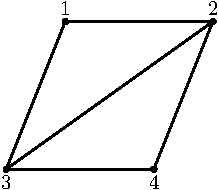
\includegraphics{gr-kim1}
  \caption{A sample figure}%
  \label{fig:fig1}
\end{figure}


\section{Code Listing}


See \autoref{lst:example}.

\begin{lstlisting}[float, floatplacement=!h, language=C, caption= {An Example For
  Code Listing}, label={lst:example}]
void main() {
  char x[16];
  read(stdin, x, 16);

  if (x[0] == 'A' && x[1] == 'B') {
      if (x[2] >= 'a') {
        if (x[2] <= 'z') {
           format1(x);
        } else {
          goto failure;
        }
      } else {
        if (x[2] >= 'A' && x[2] <= 'Z') {
           format2(x);
        } else {
           goto failure;
        }
      }
  }
failure:
  error();
}
\end{lstlisting}


\section{\LaTeX-related information}

\subsection{Input reading rules}

\LaTeX\ uses the following rules when reading input:
\begin{itemize}
  \item the end of a line is equivalent to a space
  \item spaces at the beginning of a line are ignored
\end{itemize}

The itemize environment takes lots of space---sometimes
I like to compress the layuot as shown below.

\subsection{Input preparation conventions}

I've used \LaTeX\ over~30 years
and use these personal conventions
to prepare input.
Using these conventions leads
to many short lines,
but I find those easier
to read and edit.
Do whatever works best for you.

\I2 start input lines with\\
  \I3 the first word of a sentence\\
  \I3 \verb+(+\\
  \I3 \verb+and+\\
  \I3 \verb+but+\\
  \I3 \verb+or+\\
  \I3 \verb+to+

\NL
\I2 end input lines with\\
  \I3 sentence-ending periods\\
  \I3 phrase-ending commas\\
  \I3 phrase-ending colons\\
  \I3 phrase-ending semicolons\\
  \I3 \verb+)+\\
  \I3 \verb+\\[+\textit{dimension}\verb+]+\\
  \I3 \verb+\\+

\NL
\I2 put these on a line of their own\\
  \I3 \verb+\begin{+\textit{environment name}\verb+}+\\
  \I3 \verb+\end{+\textit{environment name}\verb+}+\\
  \I3 short parenthetical remark


